\chapter{Limits of Direct (Deep) Reinforcement Learning of Decision Tree Policies}
In this chapter, we reproduce the algorithms presented in (cite). In particular, we attempt to reproduce the results from Table (cite) in which authors use deep reinforcement learning to directly learn a detph-2 decision tree for the CartPole control (cite).
We run the \textit{same} algorithms using the \textit{same} hyperparameters when possible.
Surprisingly, we are unable to reproduce their results. Even after searching for different hyperparameters, we are unable to learn decision tree policies for CartPole with reinforcement learning. 
In this chapter we provide a first set of failure modes for the direct reinforcement learning of decision tree policies and only in the next chapter will we provide more grounded insights.
(MAYBE ADD CARTPOLE FIG)
\section{Reproducing ``Iterative Bounding MDPs: Learning Interpretable Policies via Non-Interpretable Methods''}
In (cite), authors formulate an Iterative Bounding Markov Decision Process (cite) for the learning of a depth-2 decision tree policy when the base MDP is CartPole (cite).
Then they use reinforcement learning to learn a partially-observable policy from which they can extract a decision tree using Alg 6 (cite). 

Authors propose two tricks to improve learning: 1) limit the tree depth, and 2), parametric information gathering actions that adapt to the state.

\subsection{IBMDP formulation}
As described in (cite), given a base MDP $\mathcal{M}\langle S, A, R, T, T_0\rangle$, to define an IBMDP $\mathcal{M}_{IB}\langle S, O, A, A_{\info}, R, \zeta, T, T_0, T_{info}\rangle$ given a base MDP, the user needs to provide the set of information gathering actions $A_{info}$ and the reward $\zeta$ for taking those.
The observation space of the IBMDP $O$ and the deterministic transitions $T_{info}$ are induced from the given hyperparameters $A_{info}, \zeta$.

Authors propose a to parametrize the set of IGAs with $i \times p$ actions $\langle v_k, i \rangle$ with $v_k$ depending on the current observation $o=(L'_1, U'_1, \dots, L'_i, U'_i, \dots, L'_n, U'_n)$: $v_k = \frac{k(U'_i - L'_i)}{p+1}$.
This parametric IGAs space keeps the discrete IBMDP action space at a reasonable size while providing a learning agent with very veried tests.

For example, if we define an IBMDP with $p=3$ for the grid-world MDP of the previous chapter, at every time step the agent can take one of six actions. 
At $t=0$, recall that $o_0=(0, 2, 0, 2)$, so if an agent takes, e.g., IGA $\langle v_2, 2 \rangle$, the effective IGA is $\langle v_2=\frac{k(2-0)}{3+1}, i \rangle = \langle 1, 2 \rangle$ which in turn effectively corresponds to a test node ``$y \leq 1$?'' for a decisision tre policy acting in the grid-world.
If the base state has $y$ value $0.5$, then the next observation at $t=1$ is $o_1=(0, 2, 0, 1)$. Now, if the agent were to take the same IGA $\langle v_2, 2 \rangle$ again, it would be effectively $\langle v_2=\frac{k(1-0)}{3+1}, i \rangle = \langle 0.5, 2 \rangle$. 
This would give the next observation at $t=2$ $o_1=(0, 2, 0, 0.5)$ and so on \dots. 

Furthermore, akin to the supervised learning setting (cite), author propose to regularize the learned decision tree policy with a maximum depth parameter $D$.
Unfortunately, authors did not describe as they implemented the depth control in their work, hence we have to try different approaches to reproduce their results.

To control the tree depth during learning we can either penalize the agent everytime it takes more than $D$ IGAs since the last base action, or we could send a termination signal to the agent. This approach interupts the trajectory: the agent stops acting. Howver the latter, in theory, breaks the MDP formalism as a termination signal is different from an absorbing state.
The penalization approaches can also break the MDP formalism because the reward function now depends on time. We will try both approaches in our experiments.


\subsection{Deep Reinforcement Learning algorithms}
Authors of (cite) use two deep reinforcement learning baselines to which they apply some modifications in order to learn partially-observable policies from feature bounds to information gathering actions and base actions.
The first algorithm is the proximal policy optimization algorithm (PPO)(cite)(algo). This algorithm can be seen as a deep learning version of the Policy Gradient Algorithm (cite). 
The key modification to learn policies in IBMDPs that are equivalent to trees is to train a neural network policy $O\rightarrow A\cup A_{info}$ rather than a policy $S\times O\rightarrow A\cup A_{info}$ like in the traditional MDP setting.
The value function is still approximated by a neural network $S \times O \rightarrow A\cup A_{info}$.

The second deep reinforcement learning algorithm used is the deep Q-networks algorithm (DQN) (cite); a deep learning version of the Q-learning algorithm Alg (cite).
A similar modification is done to DQN to work with partially observable policy. The trained $Q$-function is approximated with a neural network $O\rightarrow A\cup A_{info}$ rather than $S\times O\rightarrow A\cup A_{info}$.
In this modified DQN, the temporal difference error target for the $Q$-function $O\rightarrow A\cup A_{info}$ is approximated by a neural network $S\times O\rightarrow A\cup A_{info}$ that is in turn trained by bootstrapping the temporal difference error with itself.

\begin{figure}
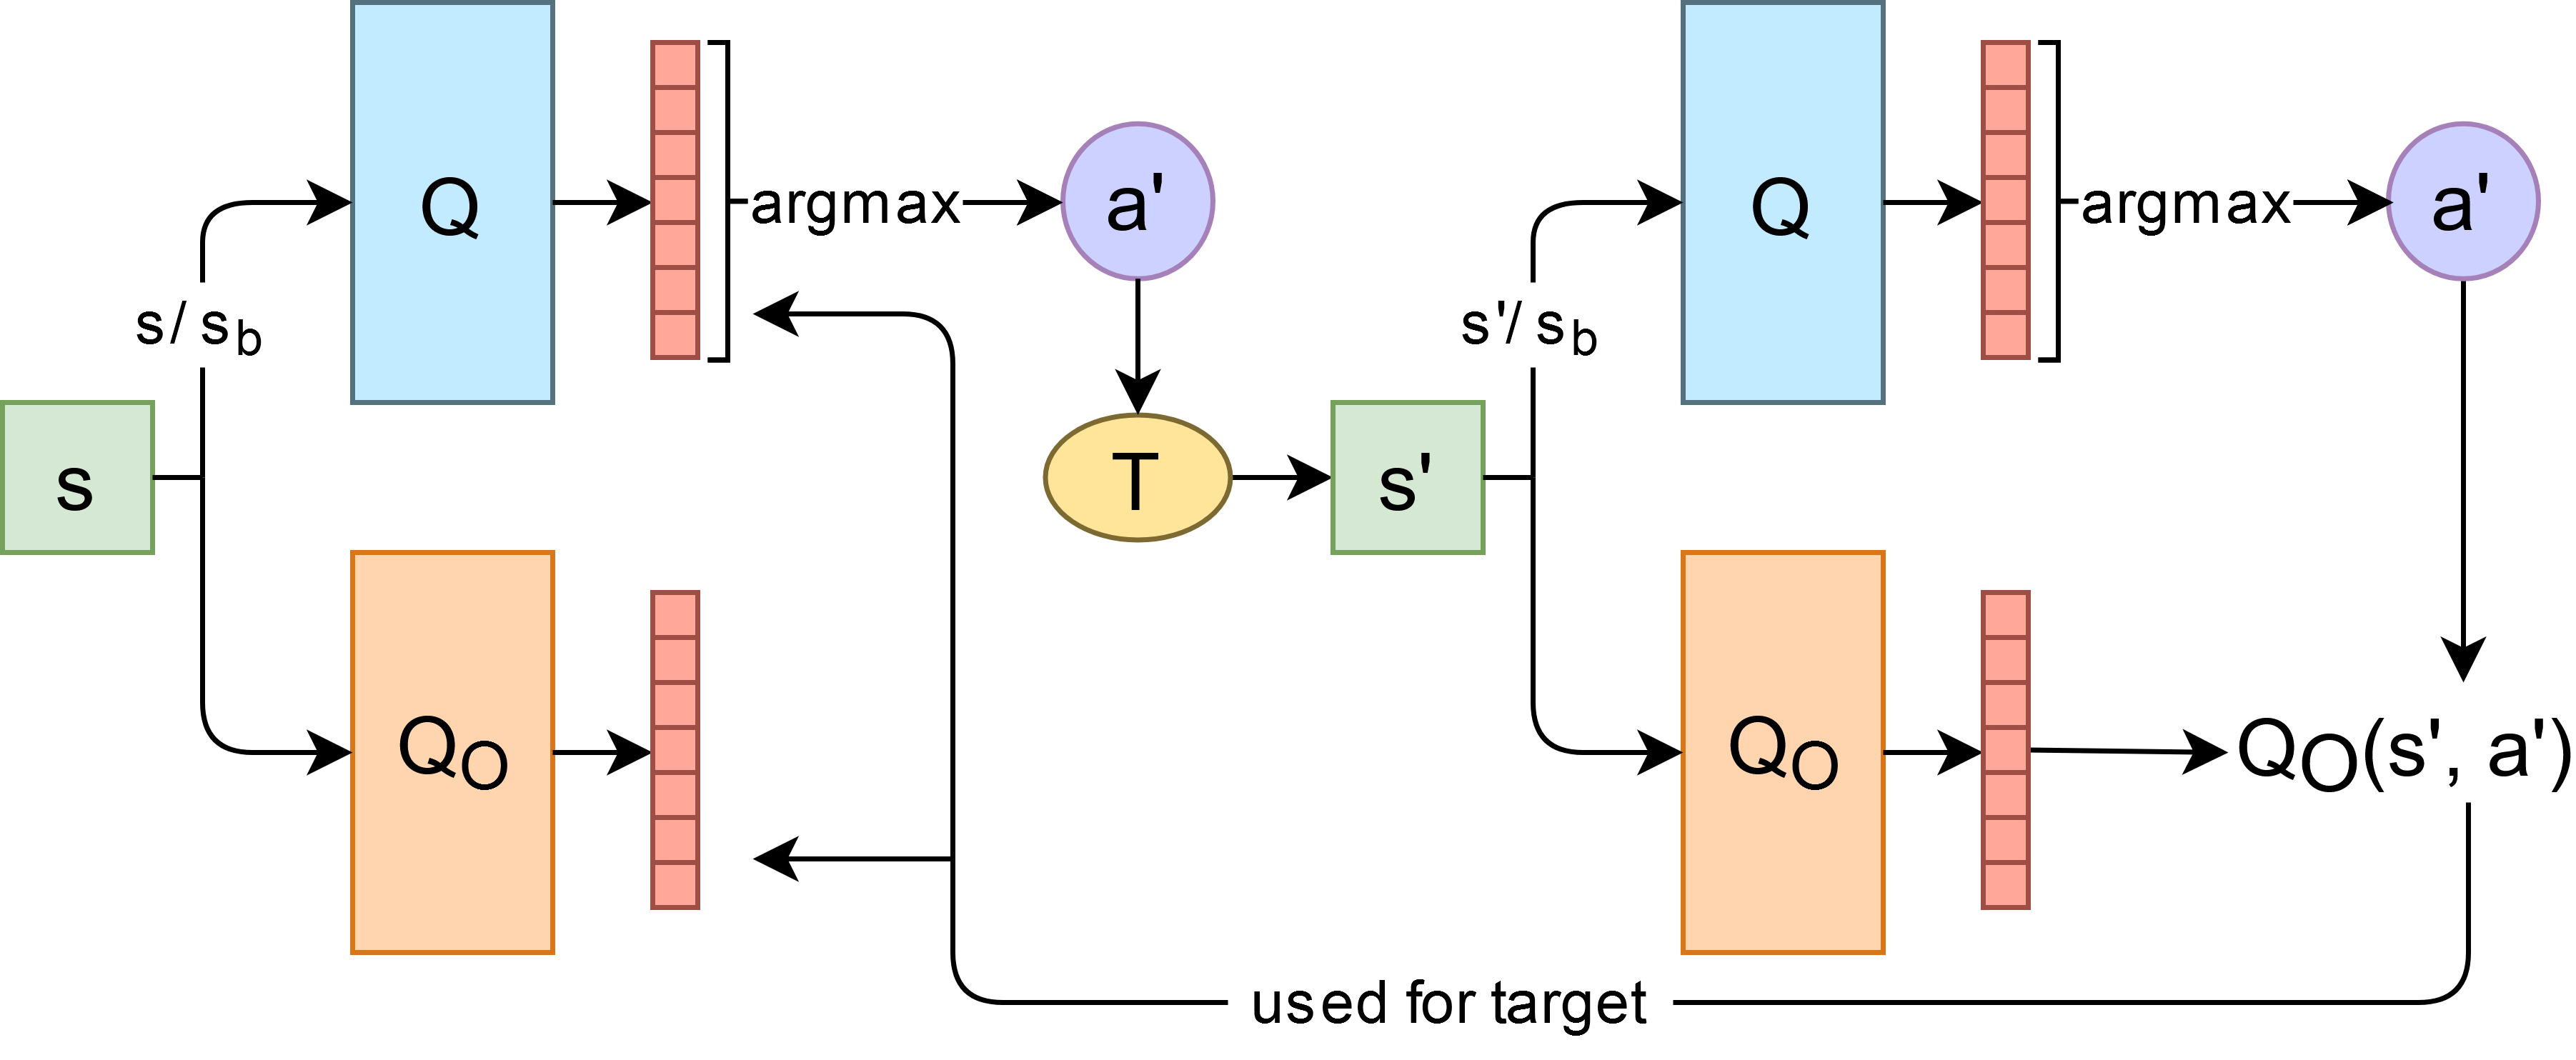
\includegraphics[width=1\textwidth]{images/images_part1/mnamenew.png}
\caption{One update of the modified DQN from (cite).}
\end{figure}

Those two variants of DQN and PPO have first been introduced in (PINTO) for robotics task and later studied theoretically to solve POMDPs (cite) in Baisero's work.
Baisero coined those approaches asymmetric reinforcement learning for POMDPs as an agent accesses full state information during the learning of a partially observable policy, hence using ``asymmetric'' information.
We study the connections between, learning decision tree policies for MDPs, and, POMDPs, extensively in the next chapter but for now we focus on reproducing the original results from (cite) in which POMDPs and asymmetric RL were not mentioned. 

Next, we present the precise experimental setup we use to reproduce the work of (cite) in order to study deep reinforcement learning of decision tree policies for the CartPole MDP.

\section{Experimental setup}


\section{Results}
\begin{figure}
    \centering
    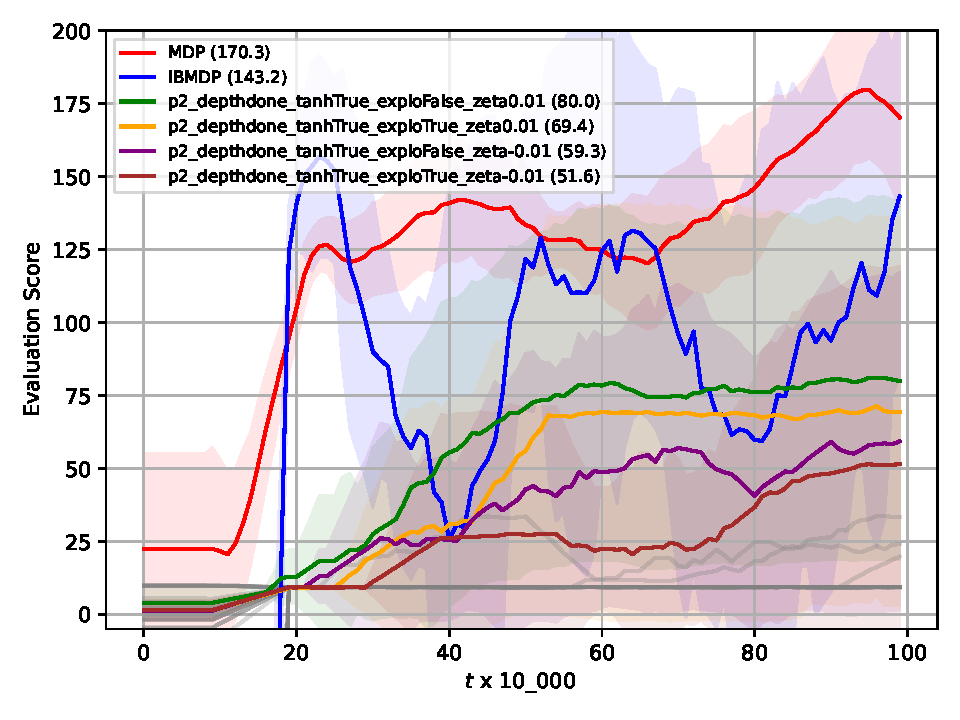
\includegraphics[width=0.8\textwidth]{images/images_part1/dqn.pdf}
    \caption{Custard DQN (cite) on CartPole.}
\end{figure}

\begin{figure}
    \centering
    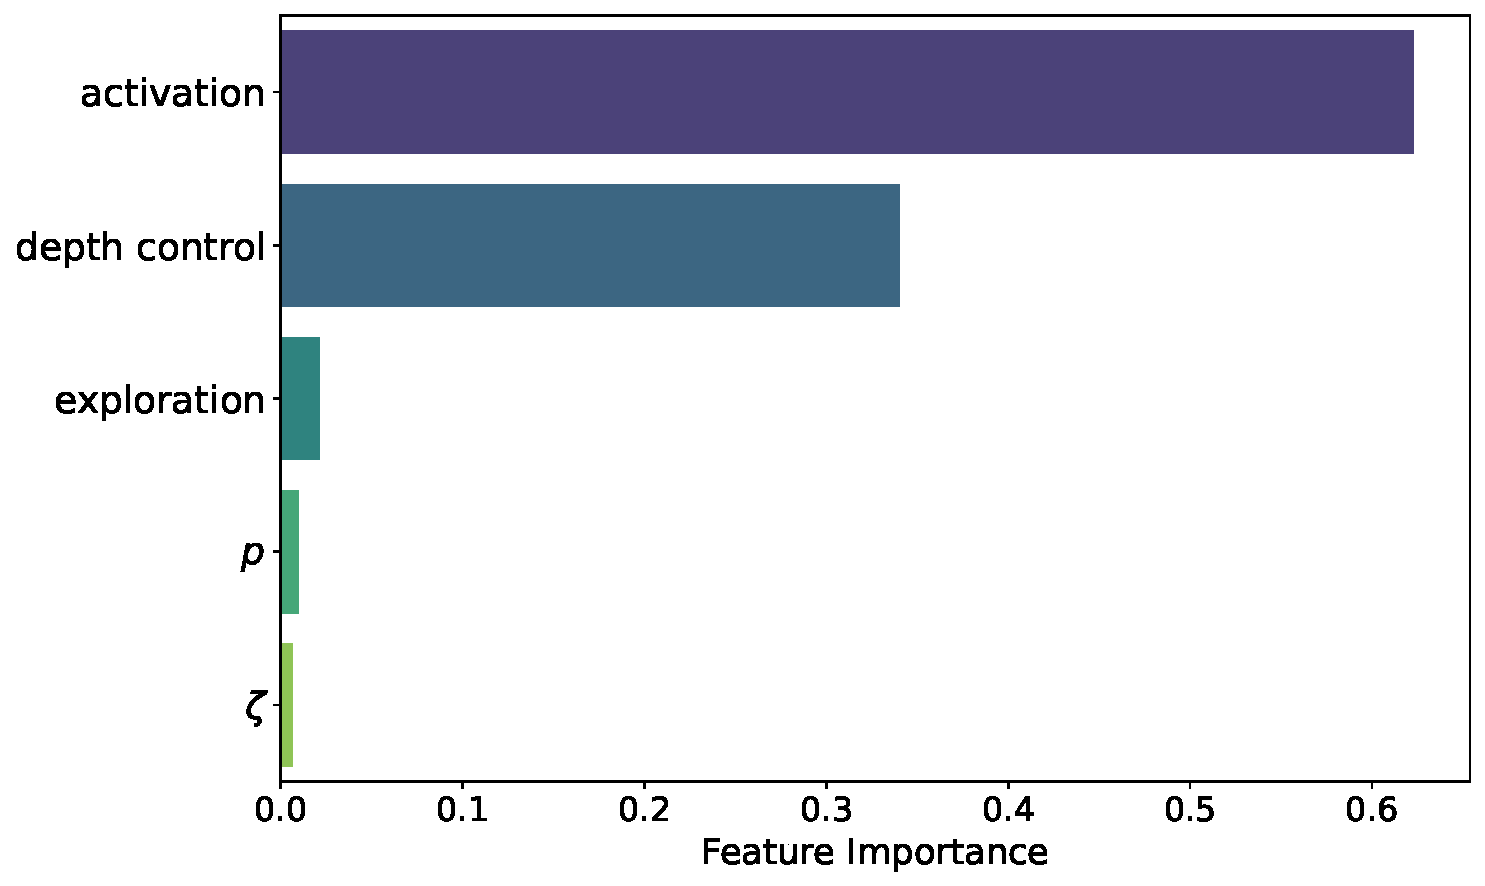
\includegraphics[width=0.8\textwidth]{images/images_part1/hyperparameter_importance_dqn.pdf}
    \caption{Custard DQN (cite) on CartPole.}
\end{figure}

\begin{figure}
    \centering
    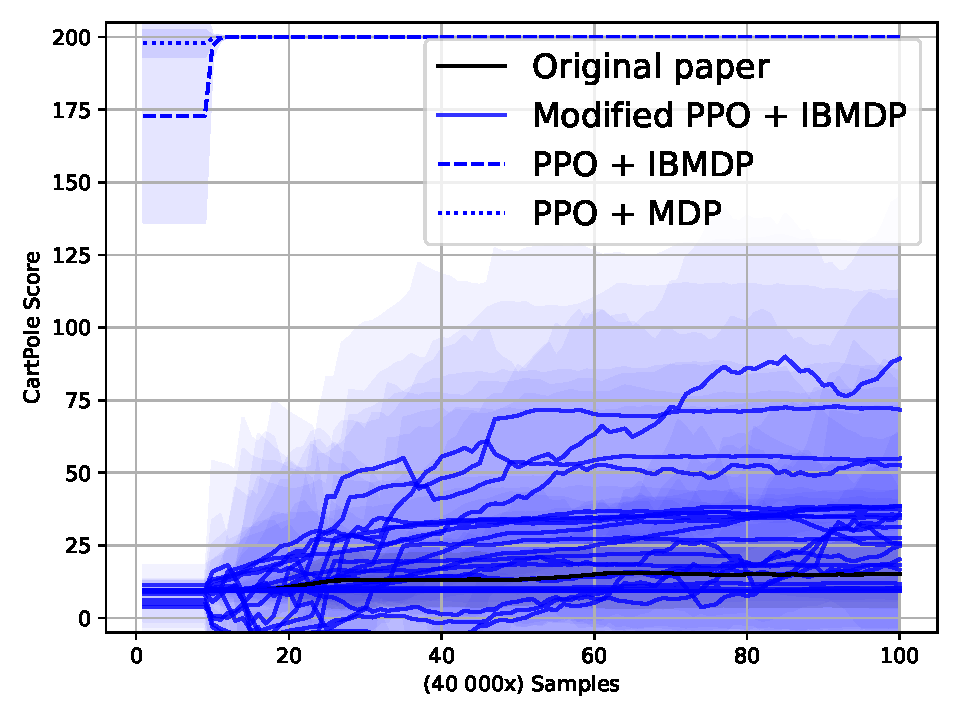
\includegraphics[width=0.8\textwidth]{images/images_part1/ppo.pdf}
    \caption{Custard PPO on CartPole}
\end{figure}

\begin{figure}
    \centering
    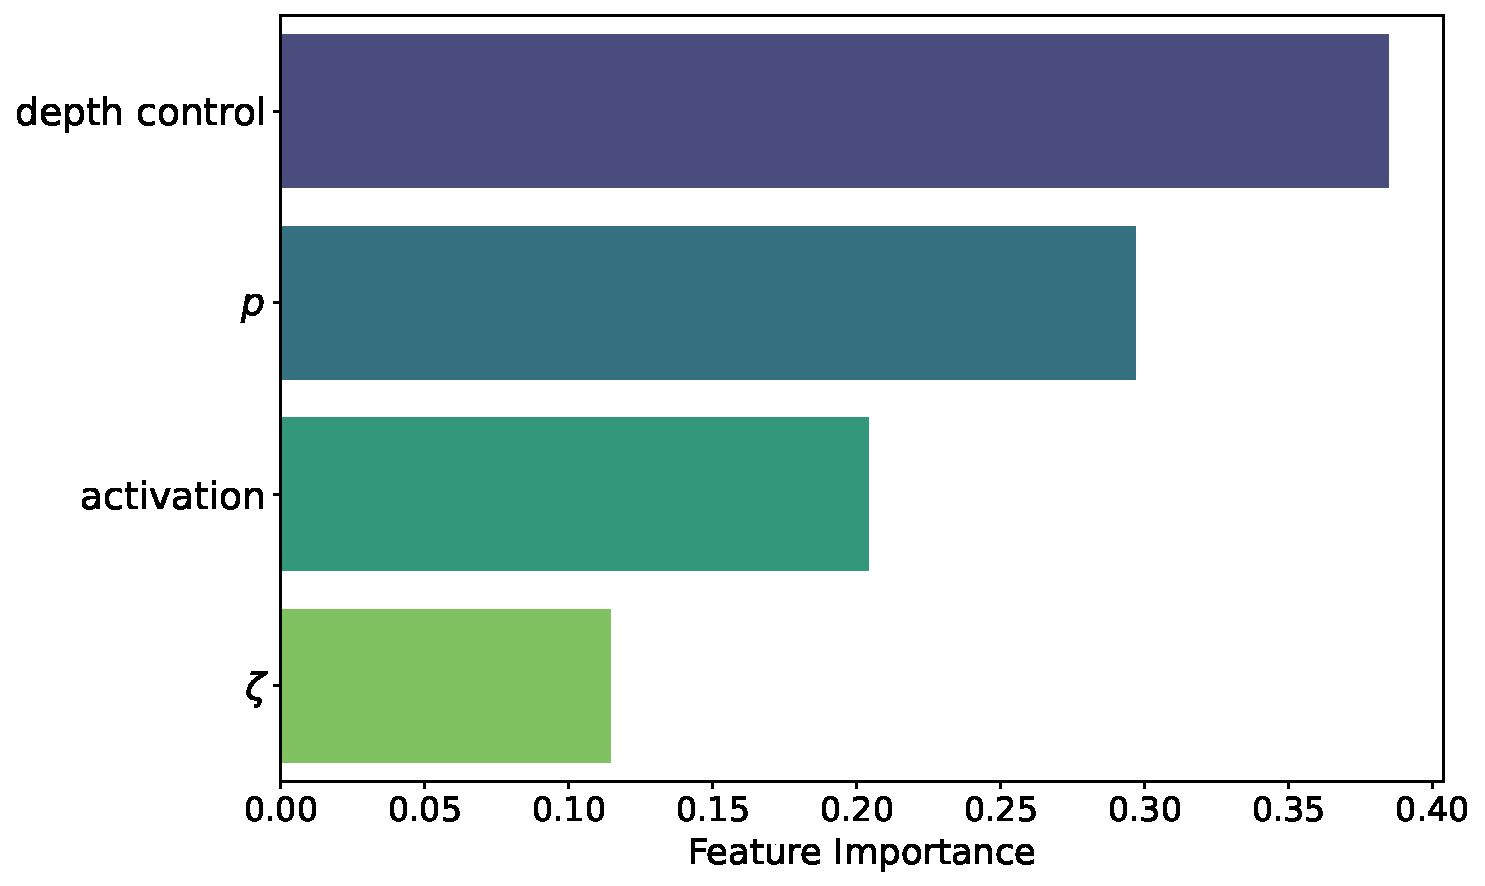
\includegraphics[width=0.8\textwidth]{images/images_part1/hyperparameter_importance_ppo.pdf}
    \caption{Custard DQN (cite) on CartPole.}
\end{figure}


\section{Discussion}
We have shown that compared to learning non-interpretable policies for both the base MDP and the associated IBMDP, learning partially observable policies in IBMDP is very difficult even when learning policies corresponding to depth-2 decision trees for the simple CartPole task.
In the next chapter we down scale the learning algorithms to highlight the connexions between the above challenges and POMDP hardness results.